\documentclass{ieeeaccess}
\usepackage{cite}
\usepackage{amsmath,amssymb,amsfonts}
\usepackage{graphicx}
\usepackage{textcomp}
\usepackage{booktabs}
\usepackage{bm}
\usepackage{xcolor}
% table rows generated by figs/bench_tables.py; primitive \input so that rules inside the rows stay legal
\makeatletter\newcommand{\rows}[1]{\@@input #1 }\makeatother
\makeatletter
\AtBeginDocument{\DeclareMathVersion{bold}
\SetSymbolFont{operators}{bold}{T1}{times}{b}{n}
\SetSymbolFont{NewLetters}{bold}{T1}{times}{b}{it}
\SetMathAlphabet{\mathrm}{bold}{T1}{times}{b}{n}
\SetMathAlphabet{\mathit}{bold}{T1}{times}{b}{it}
\SetMathAlphabet{\mathbf}{bold}{T1}{times}{b}{n}
\SetMathAlphabet{\mathtt}{bold}{OT1}{pcr}{b}{n}
\SetSymbolFont{symbols}{bold}{OMS}{cmsy}{b}{n}
\renewcommand\boldmath{\@nomath\boldmath\mathversion{bold}}}
\makeatother

\begin{document}
\history{Date of publication xxxx 00, 0000, date of current version xxxx 00, 0000.}
\doi{10.1109/ACCESS.2024.0429000}

\title{DANG: Prototype-Anchored Frozen DINOv3 Features for Generalizable Polyp Segmentation}
\author{\uppercase{Dang Thanh Tuan}\authorrefmark{1}
AND \uppercase{Le Phu-Nguyen}\authorrefmark{2}}

\address[1]{Department of Information Technology, FPT University, Ho Chi Minh City, Vietnam (e-mail: tuandtse196418@fpt.edu.vn)}
\address[2]{Faculty of Electrical and Electronics Engineering, Vietnam Aerospace University, Ho Chi Minh City, Vietnam (e-mail: nguyenlp@vaa.edu.vn)}

\markboth
{Dang and Le: DANG: Prototype-Anchored Frozen DINOv3 Features for Polyp Segmentation}
{Dang and Le: DANG: Prototype-Anchored Frozen DINOv3 Features for Polyp Segmentation}

\corresp{Corresponding author: Le Phu-Nguyen (e-mail: nguyenlp@vaa.edu.vn).}

\begin{abstract}
Polyp segmentation networks score well on the colonoscopy centres they are trained on but lose accuracy on frames from other centres and devices. We present DANG, a segmentation network built on a frozen DINOv3 ViT-S/16 foundation model with convolutional low-rank adapters. DANG reads tokens from four depths of the frozen encoder, arranges them into a four-scale pyramid decoded by a scale-aware decoder, and adds a dual-prototype margin head that scores every token against learned foreground and background prototypes and image-specific self-support centroids. Of its $23.5$M parameters only $1.9$M are trained. We train on the standard $1{,}450$-image Kvasir-SEG and CVC-ClinicDB split and test on the five standard test sets, on $1{,}399$ deduplicated frames from the six centres of PolypGen and, as a held-out final test, on $1{,}376$ frames of PolypDB. PraNet, Polyp-PVT, PraNet-V2 and SegDINO, which uses the same frozen DINOv3 encoder, are retrained from their official code with the settings of their papers, every model is evaluated at its final epoch with one evaluator, and all results are means over five seeds with paired tests. On the three cohorts our claims rest on, DANG reaches $80.7$, $82.7$ and $84.2\%$ mean Dice on CVC-ColonDB, ETIS-LaribPolypDB and PolypGen, against $80.9$, $75.5$ and $81.4\%$ for the best retrained model on each: a tie on CVC-ColonDB and gains of $7.3$ and $2.7$ points that are significant against every compared model after Holm correction. On PolypDB, which was not used for any design decision, it reaches $89.8\%$ against $86.7\%$ for the best retrained model. On the in-domain CVC-ClinicDB test set it trails Polyp-PVT by $3.2$ points. A batch-1 frame takes $9.3$~ms on an NVIDIA T4 with CUDA graphs, less than Polyp-PVT and PraNet-V2.
\end{abstract}

\begin{keywords}
Colonoscopy, deep learning, domain generalization, foundation models, medical image segmentation, parameter-efficient fine-tuning, polyp segmentation, prototype learning.
\end{keywords}

\titlepgskip=-21pt

\maketitle

\section{Introduction}
\label{sec:introduction}
\PARstart{C}{olorectal} cancer is the third most common cancer and the second leading cause of cancer death worldwide~\cite{sung2021globocan}, and removing adenomatous polyps during colonoscopy lowers colorectal-cancer mortality~\cite{zauber2012polypectomy}. Pixel-level polyp segmentation supports this by delineating lesion margins. The standard benchmark trains on $1{,}450$ frames from two centres, Kvasir-SEG~\cite{jha2020kvasir} and CVC-ClinicDB, and tests on five public sets~\cite{fan2020pranet}. On the two in-domain test sets current models exceed $90\%$ mean Dice; on CVC-ColonDB~\cite{tajbakhsh2015automated} and ETIS-LaribPolypDB~\cite{silva2014toward}, which come from other centres and cameras, the same models lose $10$--$25$ points (Table~\ref{tab:main}). Generalization to unseen centres, not in-domain accuracy, is the open problem.

Vision foundation models such as DINOv2~\cite{oquab2024dinov2} and DINOv3~\cite{simeoni2025dinov3} are trained on very large image collections and transfer across domains, which makes them natural encoders for this problem. Keeping such an encoder frozen also keeps training cheap and the trainable part small. SegDINO~\cite{yang2025segdino} pairs a frozen DINOv3 with a light decoder; under our protocol, however, it reaches only $43.2\%$ mean Dice on ETIS (Table~\ref{tab:main}). A frozen encoder trained on natural images does not see colonoscopy frames, and its $16$-pixel patch grid is coarser than lesion boundaries, so how the frozen features are adapted and decoded decides whether a frozen foundation model helps.

\begin{figure*}[!t]
  \centering
  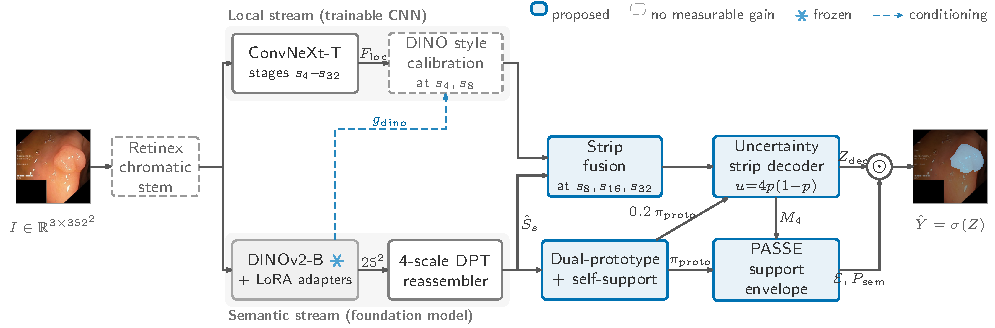
\includegraphics[width=\linewidth]{../figs/arch_diagram.pdf}
  \caption{\textbf{DANG decodes a frozen DINOv3 encoder through a token pyramid and a prototype margin head.} A $352\times352$ frame is resized to $448\times448$ and encoded by a frozen DINOv3 ViT-S/16 whose $12$ blocks carry trained Conv-LoRA adapters. Tokens from blocks $3$, $6$, $9$ and $12$ are projected to $192$ channels on the $28\times28$ grid. The token pyramid assigns one depth to each stride ($s_4$--$s_{32}$) and the scale-aware decoder fuses them top-down into the logit $Z_{\text{SAD}}$. The dual-prototype margin head (the proposed component, blue) turns the three deepest maps into the margin map $\pi_{\text{proto}}$, which is added to $Z_{\text{SAD}}$ with weight $0.2$. Dashed: heads used only for deep supervision during training. Thumbnails: a Kvasir test frame and its ground-truth mask, for illustration only.}
  \label{fig:arch}
\end{figure*}

We present \textbf{DANG} (Figure~\ref{fig:arch}) and make three contributions:
\begin{itemize}
  \item \textbf{A frozen-foundation-model segmenter with a prototype margin head.} DANG adapts a frozen DINOv3 ViT-S/16 with convolutional low-rank adapters, decodes a token pyramid with a scale-aware decoder, and adds a dual-prototype margin head with test-time self-support. It trains $1.9$M of its $23.5$M parameters and needs no convolutional backbone.
  \item \textbf{A controlled benchmark.} The standard training split; the five standard test sets kept as published; two deduplicated multi-centre cohorts, PolypGen~\cite{ali2023polypgen} and PolypDB~\cite{jha2024polypdb}, the latter held out as a final test; four published models retrained from their official code; final-epoch checkpoints, one evaluator, five seeds and paired tests with multiplicity correction.
  \item \textbf{A decoder comparison.} On the same frozen encoder and token pyramid we compare three decoders over five seeds and report what each costs in latency on an NVIDIA T4.
\end{itemize}

\section{Related Work}
\paragraph{Polyp segmentation.} Architectures progressed from U-Net~\cite{ronneberger2015unet} and UNet++~\cite{zhou2018unetplusplus} to reverse-attention networks: PraNet~\cite{fan2020pranet} mines boundary cues with parallel partial decoders and reverse attention, and CaraNet~\cite{lou2022caranet} adds axial context for small objects. Transformer encoders improved multi-centre generalization in Polyp-PVT~\cite{dong2021polyp} and TransFuse~\cite{zhang2021transfuse}, and EMCAD~\cite{rahman2024emcad} pairs a PVTv2 encoder with an efficient multi-scale convolutional attention decoder. Recent models refine the decoder further: PraNet-V2~\cite{hu2026pranetv2} supervises the background explicitly inside reverse attention, ASGNet~\cite{sun2026asgnet} guides ResNet or PVTv2 features with an adaptive spectral filter, and CSG-Mamba~\cite{wang2026csgmamba} adds convolutional gating to a vision state-space U-Net. Their reported gains are hard to compare: an audit of $27$ polyp segmentation papers~\cite{urooj2026metrics} found at least five incompatible train/test splits of the same datasets, and $26$ of the papers reported no significance test. Label-efficient work on polyps has mostly been semi-supervised; FPGM~\cite{xi2025fpgm}, for example, uses a frequency prior on polyp edges to augment unlabelled images and improve generalization to new centres.

\paragraph{Foundation models for polyps.} SAM applied without prompts segments polyps poorly~\cite{zhou2023samPolyps}, and MedSAM~\cite{ma2024medsam} fine-tunes SAM on a large medical corpus but requires box prompts. SAM~3 is being adapted in the same way: Medical SAM3~\cite{jiang2026medsam3} fully fine-tunes it on $33$ medical datasets, SAM3-Adapter~\cite{chen2025sam3adapter} trains lightweight adapters, and HAT-SAM3~\cite{li2026hatsam3} adapts it to colonoscopy with a highlight-aware boundary regulariser. SAM-Mamba~\cite{dutta2024sammamba} and SAM-MaGuP~\cite{dutta2025sammagup} adapt SAM with Mamba-based priors for zero-shot polyp generalization, at about $103$M parameters and $423$~GFLOPs~\cite{agnihotri2026litebound}. A second line distils foundation models into small networks: Polyp-DiFoM~\cite{agnihotri2025difom}, LiteBounD~\cite{agnihotri2026litebound} and Lite-$\pi$~\cite{agnihotri2026litepi}. Closest to DANG, SegDINO~\cite{yang2025segdino} keeps a DINOv3 encoder~\cite{simeoni2025dinov3} frozen and decodes multi-depth tokens with a light head, and its extended version~\cite{yang2026segdino} arranges the tokens into a multi-scale pyramid with a scale-aware decoder. DANG builds on this pyramid and decoder, adds trained adapters and a prototype margin head, and keeps the foundation model at inference without distillation.

\paragraph{Prototype-based segmentation.} Few-shot semantic segmentation classifies query pixels by their similarity to class prototypes computed from support images~\cite{wang2019panet}. Self-support prototypes~\cite{fan2022ssp} are built from confident features of the query image itself, which narrows the gap between support and query appearance. DANG adopts this self-support idea inside a fully supervised segmenter: learned prototypes and ground-truth anchors give a prior, and image-specific self-support centroids adapt it at test time.

\paragraph{Adapting frozen vision transformers.} Low-rank adaptation (LoRA~\cite{hu2022lora}) and its convolutional variant for SAM (Conv-LoRA~\cite{zhong2024convlora}) adapt frozen transformers with few parameters, and dense-prediction heads such as DPT~\cite{ranftl2021vision} reassemble ViT tokens from several depths into a multi-scale map. DANG uses Conv-LoRA adapters in every block of the frozen encoder and a fixed depth-to-stride assignment instead of learned reassembly.

\section{Method}
DANG maps an RGB frame $I\in\mathbb{R}^{3\times352\times352}$ to a polyp probability map $\hat Y=\sigma(Z)$ (Figure~\ref{fig:arch}); Figure~\ref{fig:modules} details its trained components. We write $X^{\uparrow n}$ for bilinear resizing of a map $X$ to $n\times n$ and $s_k$ for stride $k$ relative to the $352\times352$ input.

\begin{figure*}[!t]
  \centering
  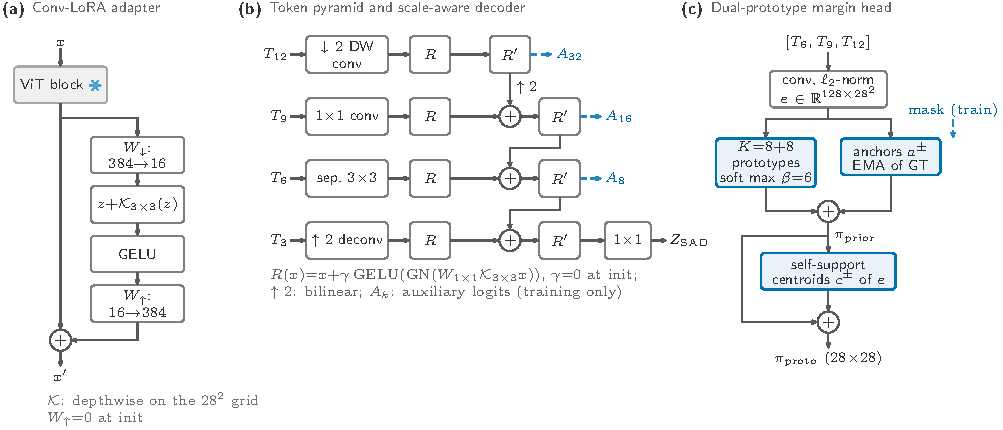
\includegraphics[width=\linewidth]{../figs/arch_modules.pdf}
  \caption{\textbf{The three trained components of DANG.} \textbf{(a)}~A Conv-LoRA adapter after each frozen ViT block (Eq.~\eqref{eq:convlora}): a rank-$16$ bottleneck with a depthwise $3\times3$ convolution on the token grid, whose up-projection starts at zero. \textbf{(b)}~The token pyramid (left column, Eq.~\eqref{eq:pyramid}) and the scale-aware decoder (Eqs.~\eqref{eq:rdb} and~\eqref{eq:topdown}): each level is refined by a residual depthwise block $R$, fused top-down with the upsampled coarser level and refined again by $R'$; auxiliary $1\times1$ heads give the deep-supervision logits $A_{32},A_{16},A_8$. \textbf{(c)}~The dual-prototype margin head (Eqs.~\eqref{eq:proto_prior} and~\eqref{eq:proto_total}): unit embeddings are scored against learned prototypes and ground-truth anchors, which are updated from the mask during training only, and the resulting prior is refined by image-specific self-support centroids.}
  \label{fig:modules}
\end{figure*}

\subsection{Frozen Encoder With Convolutional Adapters}
\label{sec:encoder}
The encoder is DINOv3 ViT-S/16~\cite{simeoni2025dinov3}, kept frozen. The frame is resized to $448\times448$ so that the $16$-pixel patches form a $28\times28$ grid of $384$-dimensional tokens. Each of the $12$ blocks is followed by a Conv-LoRA adapter~\cite{zhong2024convlora} of rank $r=16$ that acts on the block output $x$:
\begin{equation}
  x \leftarrow x + W_{\uparrow}\,\mathrm{GELU}\bigl(z+\mathcal{K}_{3\times3}(z)\bigr),\qquad z=W_{\downarrow}x,
  \label{eq:convlora}
\end{equation}
where $W_{\downarrow}\in\mathbb{R}^{r\times384}$ and $W_{\uparrow}\in\mathbb{R}^{384\times r}$ are trained, $W_{\uparrow}$ is initialised to zero so that training starts from the frozen encoder, and $\mathcal{K}_{3\times3}$ is a depthwise convolution applied to the patch tokens on the $28\times28$ grid. The adapters add $0.15$M parameters. We read the normalised patch tokens after blocks $3$, $6$, $9$ and $12$ and project each with a $1\times1$ convolution, batch normalisation and activation to a map $T_\ell\in\mathbb{R}^{192\times28\times28}$, $\ell\in\{3,6,9,12\}$.

\subsection{Token Pyramid and Scale-Aware Decoder}
\label{sec:decoder}
Following the token pyramid of the extended SegDINO~\cite{yang2026segdino}, each depth is assigned to one stride, shallow depths to fine strides:
\begin{equation}
\begin{aligned}
  P_4 &= \phi_4\bigl(\mathcal{U}(T_3^{\uparrow44})\bigr), & P_8 &= \phi_8\bigl(T_6^{\uparrow44}\bigr),\\
  P_{16} &= \phi_{16}\bigl(T_9^{\uparrow22}\bigr), & P_{32} &= \phi_{32}\bigl(\mathcal{D}(T_{12}^{\uparrow22})\bigr),
\end{aligned}
  \label{eq:pyramid}
\end{equation}
where $\mathcal{U}$ is a learned depthwise $2\times$ transposed convolution, $\mathcal{D}$ a depthwise convolution with stride $2$, and $\phi_s$ light convolution blocks (separable $3\times3$ at $s_4$ and $s_8$, $1\times1$ at $s_{16}$ and $s_{32}$). The pyramid has no convolutional backbone: all four levels come from the frozen encoder.

The scale-aware decoder of~\cite{yang2026segdino} refines each level with a residual depthwise block
\begin{equation}
  R(x)=x+\gamma\,\mathrm{GELU}\bigl(\mathrm{GN}(W_{1\times1}\,\mathcal{K}_{3\times3}(x))\bigr),
  \label{eq:rdb}
\end{equation}
with a learned scalar $\gamma$ initialised to zero and group normalisation $\mathrm{GN}$, and then fuses the levels top-down,
\begin{equation}
\begin{aligned}
  X_{32}&=R'_{32}\bigl(R_{32}(P_{32})\bigr),\\
  X_k&=R'_k\bigl(X_{2k}^{\uparrow}+R_k(P_k)\bigr),\quad k=16,8,4,
\end{aligned}
  \label{eq:topdown}
\end{equation}
where $R_k$ and $R'_k$ are separate blocks of the form of Eq.~\eqref{eq:rdb}. A $1\times1$ convolution on $X_4$ gives the decoder logit $Z_{\text{SAD}}$ at $s_4$ ($88\times88$). For deep supervision during training, $1\times1$ heads on $X_8$, $X_{16}$ and $X_{32}$ give auxiliary logits $A_8$, $A_{16}$ and $A_{32}$; they are not used at inference.

\subsection{Dual-Prototype Margin Head}
\label{sec:proto}
The head concatenates the three deepest maps $T_6$, $T_9$ and $T_{12}$, projects them with a $3\times3$ convolution block and a $1\times1$ convolution to $128$ channels, and normalises each position to a unit embedding $e_{u,v}$ on the $28\times28$ grid. It compares $e_{u,v}$ with $K=8$ learned foreground prototypes $p_k^+$ and $K=8$ background prototypes $p_k^-$ (unit vectors, orthogonally initialised), and with a foreground anchor $a^+$ and background anchor $a^-$:
\begin{align}
  \pi_{\text{prior}}(u,v) &= \tfrac{\tau}{\beta}\Bigl(\log\textstyle\sum_k e^{\beta\langle e_{u,v},p_k^+\rangle}-\log\textstyle\sum_k e^{\beta\langle e_{u,v},p_k^-\rangle}\Bigr)\nonumber\\
  &\quad + w_{\text{a}}\bigl(\langle e_{u,v},a^+\rangle-\langle e_{u,v},a^-\rangle\bigr)+b.
  \label{eq:proto_prior}
\end{align}
The log-sum-exp with fixed sharpness $\beta$ is a soft maximum over prototypes; the temperature $\tau$, the bias $b$ and the bounded anchor weight $w_{\text{a}}$ are learned. During training only, $a^\pm$ are exponential moving averages of the embeddings at positions where the ground-truth mask, average-pooled to $28\times28$, is mostly foreground or mostly background. At training and test time the head then forms image-specific self-support centroids~\cite{fan2022ssp} weighted by the prior's own confidence, $c^+=\mathrm{Norm}(\sum_{u,v}q_{u,v}^2e_{u,v})$ and $c^-=\mathrm{Norm}(\sum_{u,v}(1-q_{u,v})^2e_{u,v})$ with $q=\sigma(\pi_{\text{prior}})$, and outputs the margin map
\begin{equation}
  \pi_{\text{proto}}=\pi_{\text{prior}}+w_{\text{ss}}\bigl(\langle e,c^+\rangle-\langle e,c^-\rangle\bigr),
  \label{eq:proto_total}
\end{equation}
with a learned bounded weight $w_{\text{ss}}$. The final logit is
\begin{equation}
  Z=\bigl(Z_{\text{SAD}}+0.2\,\pi_{\text{proto}}^{\uparrow88}\bigr)^{\uparrow352}.
  \label{eq:output}
\end{equation}
The prototype margin thus enters the output as a coarse, token-level prior on top of the decoder logit. Constant values are listed in Appendix~\ref{app:impl}.

\subsection{Training Objective}
\label{sec:loss}
DANG is trained with
\begin{align}
  \mathcal{L} &= \mathcal{L}_{\text{BCE+Dice}}^{w}(Z,Y)+0.25\,\mathcal{L}_{\text{Tv}}^{w}(Z,Y)+0.1\,\mathcal{L}_{\text{far}}(Z,Y)\nonumber\\
  &\quad +\tfrac{0.25}{3}\textstyle\sum_{k\in\{8,16,32\}}\mathcal{L}_{\text{BCE+Dice}}^{w}(A_k^{\uparrow352},Y)+0.35\,\mathcal{L}_{\text{proto}}.
  \label{eq:loss}
\end{align}
Each image's terms are weighted by $w$, which grows as lesion area shrinks. The Tversky term $\mathcal{L}_{\text{Tv}}$ penalises false negatives more for small lesions. $\mathcal{L}_{\text{far}}$ is the mean predicted probability outside dilations of the ground truth. $\mathcal{L}_{\text{proto}}$ applies the cross-entropy, Dice and Tversky terms to $\pi_{\text{proto}}$ against the mask average-pooled to $28\times28$. Exact forms are in Appendix~\ref{app:impl}. During training, each image's amplitude spectrum is mixed with that of another image in the batch with probability $0.5$, keeping its phase (Fourier amplitude mix~\cite{xu2021fact}), to vary colour and illumination statistics.

\section{Experimental Setup}
\subsection{Data}
\label{sec:data}
We use the standard split~\cite{fan2020pranet}: $900$ Kvasir-SEG and $550$ CVC-ClinicDB images for training, and the five standard test sets kept exactly as published (Table~\ref{tab:data}). Because these test sets are small, we add two multi-centre cohorts. From PolypGen~\cite{ali2023polypgen} we keep $1{,}399$ of $1{,}536$ frames from its six centres, after dropping $125$ frames with empty masks and $12$ within-set duplicates. From PolypDB~\cite{jha2024polypdb} we keep $1{,}376$ frames of six centre and modality groups (white light, BLI, FICE, LCI and NBI); we drop its Norwegian white-light group, which comes from the hospital that collected Kvasir-SEG. Every kept frame is compared against all $1{,}450$ training images and the frames already kept from its own set. Two frames count as duplicates when their MD5 hashes match, or when the Pearson correlation of their $32\times32$ grey-scale thumbnails, taken after cropping the dark endoscope border, is at least $0.97$ and their masks overlap with IoU at least $0.8$. A $64$-bit difference hash was tried first and rejected because the black border dominates it on endoscopy frames. The highest thumbnail correlation of a kept frame with any training image is $0.94$ for PolypGen and $0.92$ for PolypDB.

\begin{table}[!t]
  \centering
  \caption{\textbf{Cohorts.} The five standard test sets are kept as published; PolypGen and PolypDB are deduplicated against the training images. Primary: the cohorts our claims rest on. PolypDB is the held-out final test.}
  \label{tab:data}
  \vspace{2pt}
  \setlength{\tabcolsep}{3pt}\footnotesize
  \begin{tabular}{@{}l l r l@{}}
    \toprule
    \textbf{Cohort} & \textbf{Source} & \textbf{Images} & \textbf{Role} \\
    \midrule
    Train & Kvasir-SEG + CVC-ClinicDB & 1,450 & training \\
    Kvasir & Kvasir-SEG~\cite{jha2020kvasir} & 100 & in domain \\
    ClinicDB & CVC-ClinicDB & 62 & in domain \\
    ColonDB & CVC-ColonDB~\cite{tajbakhsh2015automated} & 380 & primary \\
    ETIS & ETIS-LaribPolypDB~\cite{silva2014toward} & 196 & primary \\
    CVC-300 & EndoScene test~\cite{fan2020pranet} & 60 & reported \\
    PolypGen & PolypGen, 6 centres~\cite{ali2023polypgen} & 1,399 & primary \\
    PolypDB & PolypDB, 6 groups~\cite{jha2024polypdb} & 1,376 & final test \\
    \bottomrule
  \end{tabular}
\end{table}

We base our claims on CVC-ColonDB, ETIS and PolypGen, the three cohorts that are both external to the training centres and large enough for per-image statistics. Kvasir and ClinicDB share their training centres, and ClinicDB and CVC-300 are so small that one image moves mean Dice by $1.6$ and $1.7$ points; we report them for comparability.

\subsection{Models and Training}
\label{sec:training}
DANG is trained for $20$ epochs at $352\times352$ with batch size $16$, AdamW, linear warm-up and cosine decay, gradient clipping, mixed precision and an exponential moving average of the weights; all hyperparameters are listed in Table~\ref{tab:impl}. There is no validation split and no checkpoint selection: we evaluate the moving-average weights after the last epoch.

Published scores rest on incompatible splits and are rarely tested for significance~\cite{urooj2026metrics}, and the released training scripts of some models select checkpoints on test data. We therefore retrain the compared models instead of copying their numbers. PraNet~\cite{fan2020pranet}, Polyp-PVT~\cite{dong2021polyp} and PraNet-V2~\cite{hu2026pranetv2} are retrained from their official code with the training settings of their papers and released scripts, and SegDINO~\cite{yang2025segdino}, which uses the same frozen DINOv3 ViT-S/16 encoder as DANG, with those of its paper. Every model is evaluated at its final epoch.

\subsection{Metrics and Statistics}
\label{sec:stats}
All models are scored by one evaluator. Probabilities are resized bilinearly to the native ground-truth resolution and thresholded at $0.5$; Dice is computed per image and averaged over the images of a cohort (for PolypGen and PolypDB, over all frames of all centres). For comparison with published tables we also report the toolbox mean Dice, the Dice averaged over $256$ thresholds of the min-max-normalised probability map, which is the metric of the evaluation scripts behind PraNet, Polyp-PVT and PraNet-V2.

Five seeds ($42$--$46$) are run for every model. We test DANG against each compared model in two ways. At the seed level, a two-sided paired $t$-test compares the per-seed mean Dice of matched seeds ($n=5$). At the image level, a two-sided Wilcoxon signed-rank test~\cite{wilcoxon1945individual} compares per-image Dice averaged over the five seeds. For each compared model, Holm's procedure~\cite{holm1979simple} corrects each test over the three primary cohorts.

Inference cost is measured for all models in one process on one NVIDIA T4 at batch size $1$ and $352\times352$ input ($256\times256$ for SegDINO, its own resolution): the median of $300$ timed forward passes after $50$ warm-up passes, in FP16 autocast (eager) and with FP16 weights replayed from a CUDA graph. We also report multiply-accumulate operations (MACs) per frame and total parameters, frozen weights included.

\section{Results}

\begin{table*}[!t]
  \centering
  \caption{\textbf{Comparison with retrained published models.} Dice (\%) at threshold $0.5$, mean $\pm$ SD over $5$ seeds, final-epoch weights, one evaluator. ColonDB, ETIS and PolypGen are the primary cohorts; PolypDB is the held-out final test, run once for the selected model. \textbf{Bold}: best in column. $^{*}$: worse than DANG after Holm correction (seed-level paired $t$-test, Section~\ref{sec:stats}). Params: total parameters in millions, frozen weights included; Trained: parameters updated in training.}
  \label{tab:main}
  \vspace{2pt}
  \setlength{\tabcolsep}{4pt}\resizebox{\textwidth}{!}{%
  \begin{tabular}{l cc ccccccc}
    \toprule
    & & & \multicolumn{2}{c}{\textbf{In domain}} & \multicolumn{3}{c}{\textbf{Primary (external)}} & \textbf{External} & \textbf{Final test} \\
    \cmidrule(lr){4-5} \cmidrule(lr){6-8} \cmidrule(lr){9-9} \cmidrule(lr){10-10}
    \textbf{Model} & Params & Trained & Kvasir & ClinicDB & ColonDB & ETIS & PolypGen & CVC-300 & PolypDB \\
    \midrule
    \rows{../figs/tab_main_rows.tex}
    \bottomrule
  \end{tabular}%
  }
\end{table*}

\begin{figure*}[!t]
  \centering
  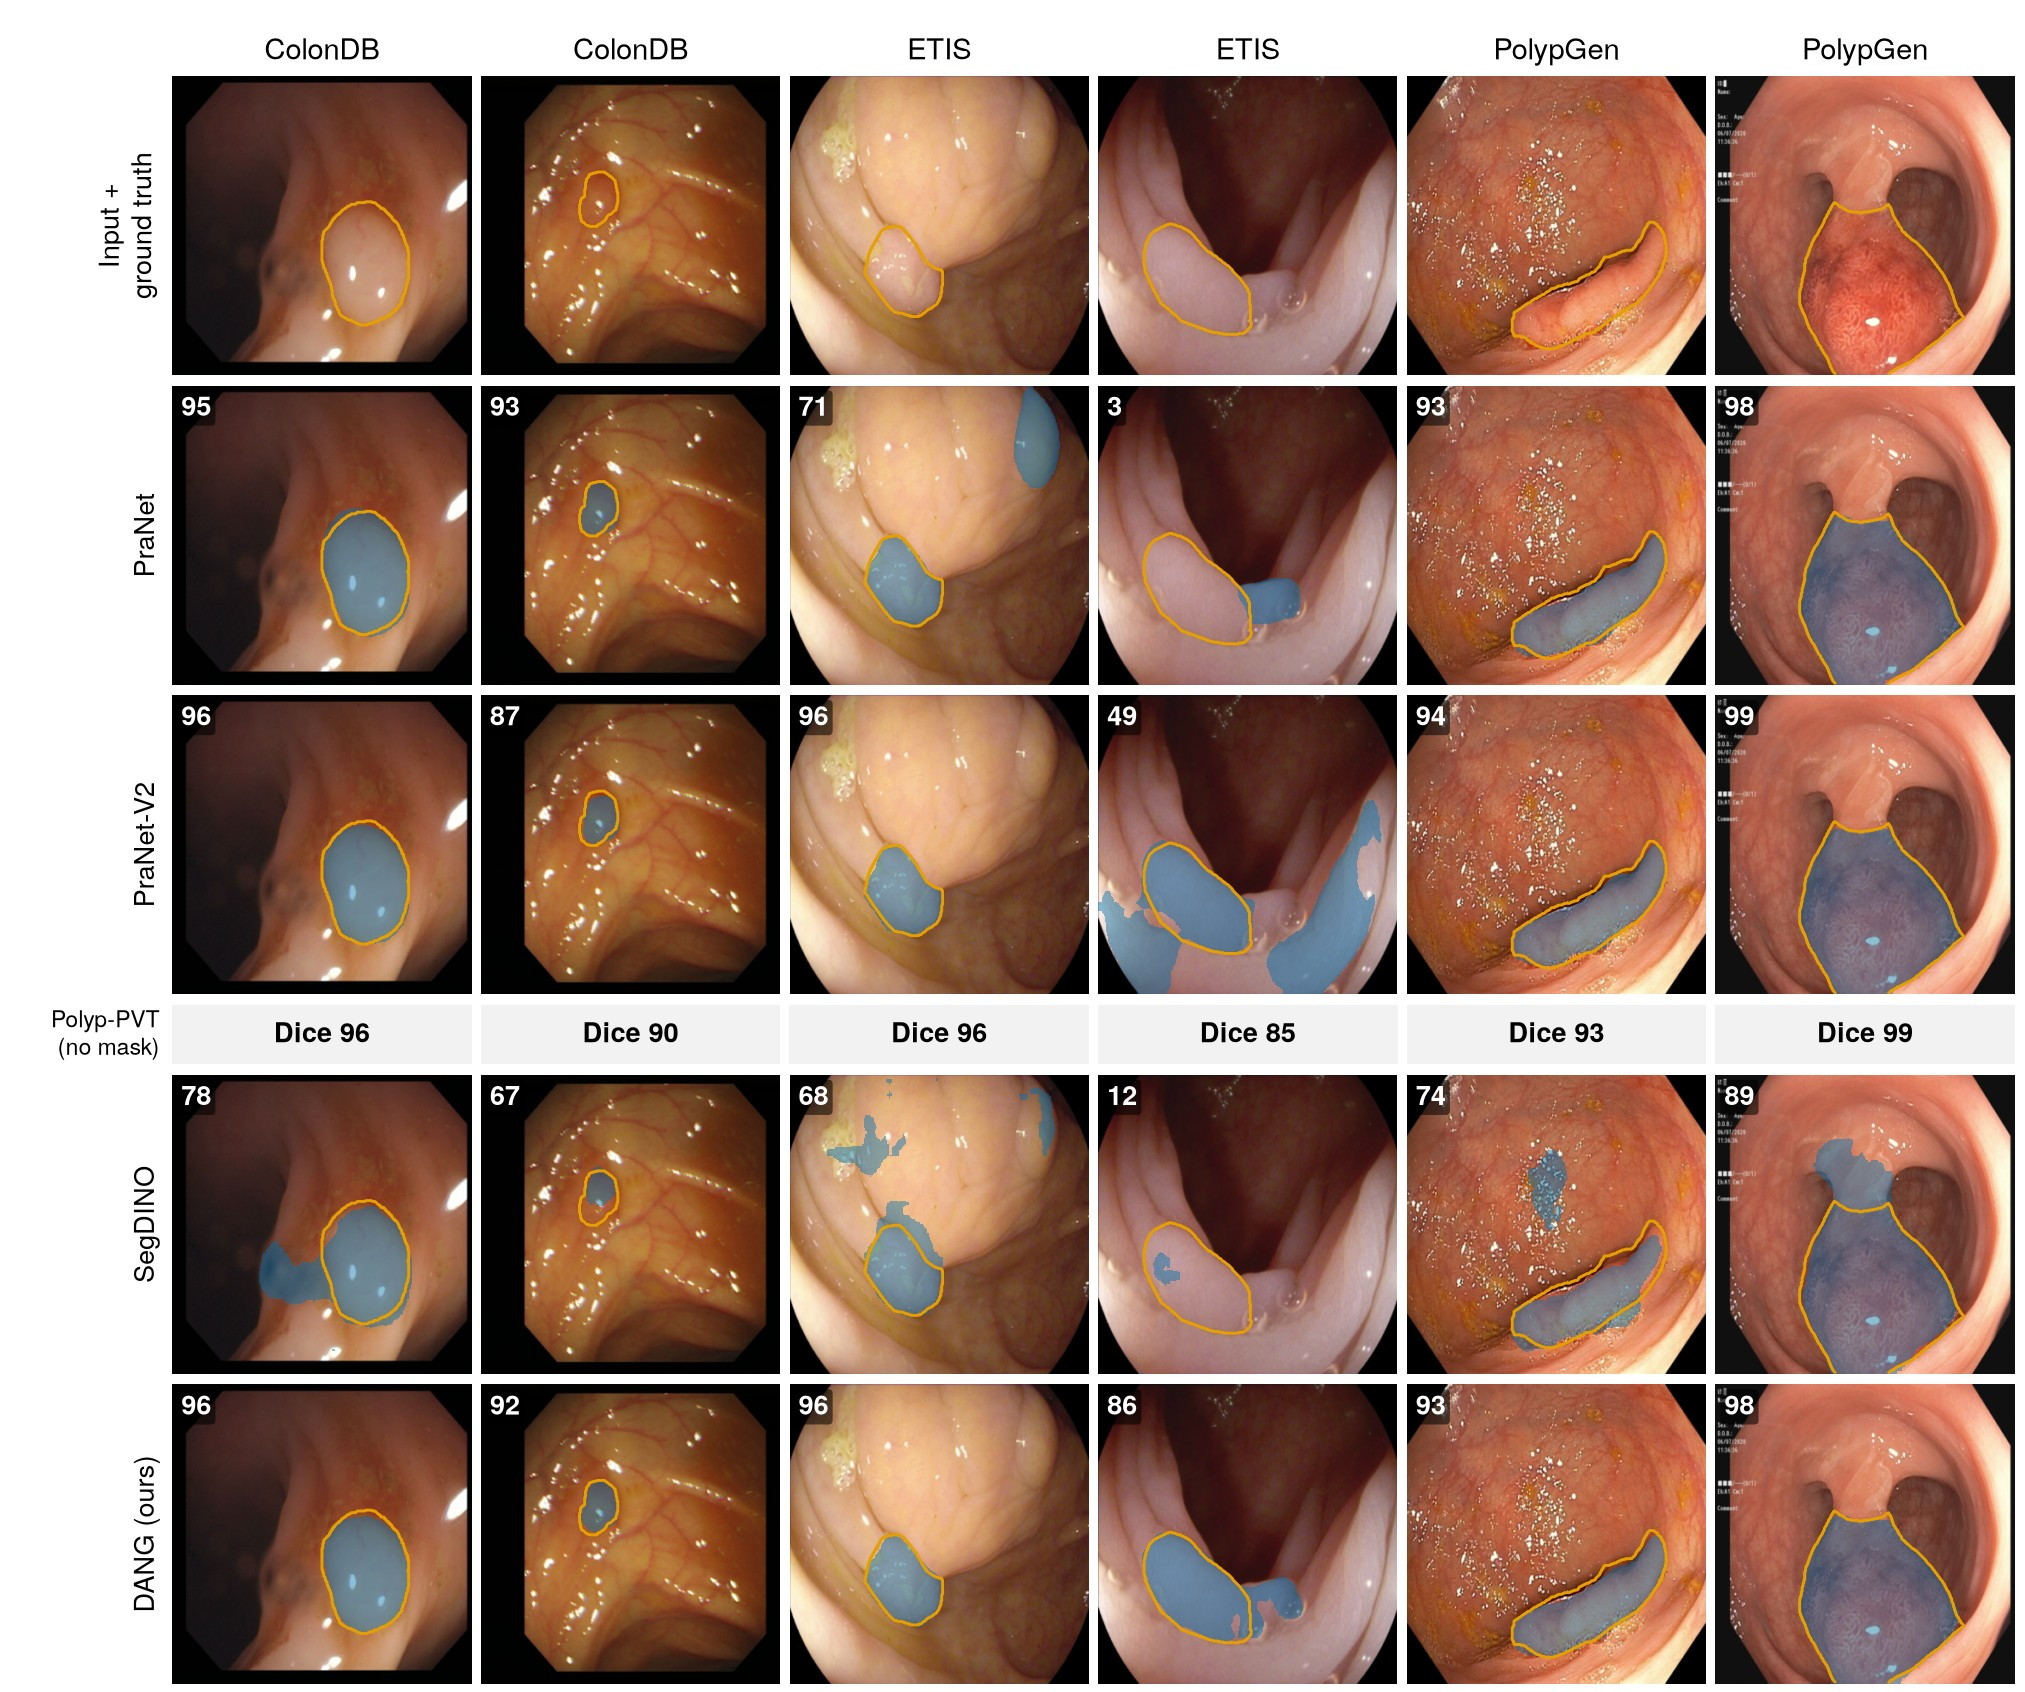
\includegraphics[width=\linewidth]{../figs/qualitative_bench.jpg}
  \caption{\textbf{Predictions on the primary cohorts, drawn at random.} Two frames per cohort, chosen by a fixed random generator among all frames (not curated); seed $42$ of each model. Orange contour: ground truth; blue fill: prediction at threshold $0.5$; number: per-image Dice (\%) at native resolution. Polyp-PVT's prediction masks were not retained; its strip gives the per-image Dice it logged for the same frames and seed.}
  \label{fig:qual}
\end{figure*}

\begin{figure*}[!t]
  \centering
  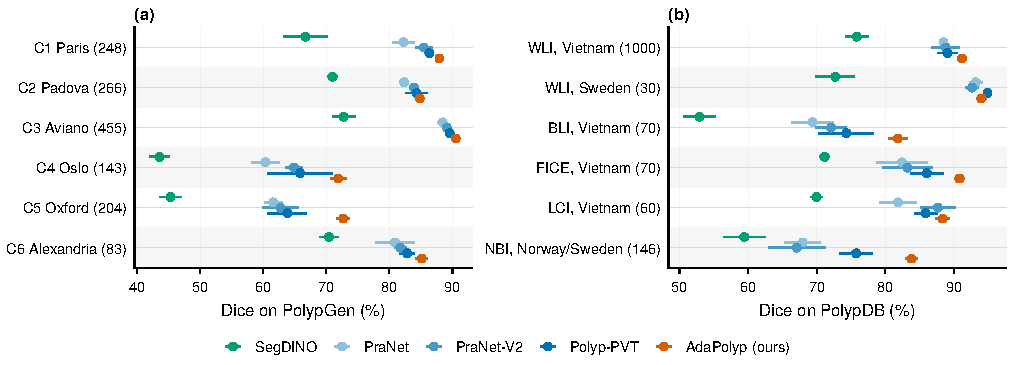
\includegraphics[width=\linewidth]{../figs/per_centre.pdf}
  \caption{\textbf{DANG gains most on the centres where every model is weakest.} Dice (\%) per centre of PolypGen \textbf{(a)} and per centre and imaging modality of PolypDB \textbf{(b)}; number of frames in parentheses. Points are means over $5$ seeds, bars $95\%$ $t$-intervals.}
  \label{fig:centre}
\end{figure*}

\subsection{Comparison With Retrained Published Models}
\label{sec:sota}
Table~\ref{tab:main} compares DANG with the four retrained models. Among them, Polyp-PVT is the strongest on ColonDB ($80.9\%$) and PolypGen ($81.4\%$), and PraNet-V2 on ETIS ($75.5\%$). DANG reaches $80.7\%$ on ColonDB, $82.7\%$ on ETIS and $84.2\%$ on PolypGen. On ColonDB it ties Polyp-PVT ($-0.2$ points); on ETIS and PolypGen it is $7.3$ and $2.7$ points above the best retrained model, with the smallest seed-to-seed SD of all models on the three primary cohorts ($0.2$--$0.7$ points). On Kvasir it is the best model ($92.2\%$, $+1.2$ points), while on ClinicDB ($89.7\%$) it is $3.2$ points below Polyp-PVT and on CVC-300 ($88.8\%$) $1.0$ point below PraNet. ClinicDB is one of the two training centres, so the models with fully fine-tuned encoders may fit it more closely; with $62$ images, one image is worth $1.6$ points, so the gap amounts to two images. On the held-out PolypDB, run once after all design decisions, DANG reaches $89.8\pm0.1\%$, $3.1$ points above Polyp-PVT ($86.7\%$), $4.4$ and $5.0$ points above PraNet-V2 and PraNet, and $17.5$ points above SegDINO; against Polyp-PVT this single pre-specified comparison is significant at the seed level (paired $t$-test, $p=0.005$) and at the image level ($p<0.001$; $713$ frames better, $662$ worse).

SegDINO, which uses the same frozen encoder with a light decoder, stays far below every other model, at $51.5\%$ on ColonDB and $43.2\%$ on ETIS. It is trained at the $256\times256$ input of its paper and without adapters, so this gap mixes input resolution and adaptation; Section~\ref{sec:ablation} compares decoders on the DANG encoder at a fixed resolution. We keep it as the reference for a frozen foundation model with a light head: DANG uses the same frozen weights and trains a comparable number of parameters ($1.9$M against $2.5$M).

\begin{table*}[!t]
  \centering
  \caption{\textbf{Paired tests of DANG against each retrained model} on the primary cohorts. $\Delta$: mean Dice difference (pp, DANG minus model) over $5$ matched seeds; $p_{\text{seed}}$: paired $t$-test over seeds; $p_{\text{img}}$: Wilcoxon signed-rank test over images on seed-averaged Dice, with the number of images on which DANG is better/worse. All $p$-values Holm-corrected over the three cohorts.}
  \label{tab:stats}
  \vspace{2pt}
  \setlength{\tabcolsep}{6pt}\footnotesize\resizebox{\textwidth}{!}{%
  \begin{tabular}{l ccc ccc ccc}
    \toprule
    & \multicolumn{3}{c}{\textbf{ColonDB} ($n=380$)} & \multicolumn{3}{c}{\textbf{ETIS} ($n=196$)} & \multicolumn{3}{c}{\textbf{PolypGen} ($n=1{,}399$)} \\
    \cmidrule(lr){2-4} \cmidrule(lr){5-7} \cmidrule(lr){8-10}
    & $\Delta$ & $p_{\text{seed}}$ & $p_{\text{img}}$ & $\Delta$ & $p_{\text{seed}}$ & $p_{\text{img}}$ & $\Delta$ & $p_{\text{seed}}$ & $p_{\text{img}}$ \\
    \midrule
    \rows{../figs/tab_stats_rows.tex}
    \bottomrule
  \end{tabular}%
  }
\end{table*}

\paragraph{Per centre.} Figure~\ref{fig:centre}a splits PolypGen by centre. DANG has the highest mean Dice on all six centres. Its margin over the best retrained model is $0.5$--$2.3$ points on Paris, Padova, Aviano and Alexandria and $6.1$ and $8.9$ points on Oslo and Oxford, the two centres on which every retrained model stays below $66\%$. On PolypDB (Figure~\ref{fig:centre}b), DANG is the best model on five of the six groups. Its gains are largest on the two virtual-chromoendoscopy modalities absent from training, narrow-band imaging ($83.8$ against $75.8\%$ for Polyp-PVT) and blue-light imaging ($81.8$ against $74.3\%$); on the $30$ Swedish white-light frames it is $0.9$ points below Polyp-PVT.

\paragraph{Examples.} Figure~\ref{fig:qual} shows six frames drawn at random from the primary cohorts. Five are segmented well by PraNet, PraNet-V2, Polyp-PVT and DANG, while SegDINO adds scattered false positives on most of them (Dice $67$--$89\%$). On the second ETIS frame PraNet finds only a fragment of the lesion (Dice $3\%$), PraNet-V2 adds large false positives on the surrounding folds ($49\%$) and SegDINO reaches $12\%$, while Polyp-PVT and DANG reach $85$ and $86\%$.

\paragraph{Statistical tests.} Table~\ref{tab:stats} gives the paired tests on the primary cohorts. On ETIS and PolypGen, DANG is better than every retrained model at the seed and the image level after Holm correction; against Polyp-PVT the seed-level adjusted $p$-values are $0.007$ and $0.031$, and DANG is better on $123$ of $196$ ETIS images (worse on $70$) and on $746$ of $1{,}399$ PolypGen frames (worse on $647$). On ColonDB, DANG is better than PraNet, PraNet-V2 and SegDINO, and statistically indistinguishable from Polyp-PVT at both levels (adjusted $p=0.72$ and $0.99$; $187$ images better, $191$ worse).

\begin{table}[!t]
  \centering
  \caption{\textbf{Toolbox mean Dice on the standard test sets} (\%), the metric of published polyp tables. Published rows are copied from the papers; $^{\ddagger}$: the released training script selects its checkpoint on test data. Our rows: mean $\pm$ SD over $5$ seeds, final-epoch weights. \textbf{Bold}: best of our rows.}
  \label{tab:toolbox}
  \vspace{2pt}
  \setlength{\tabcolsep}{2.5pt}\resizebox{\columnwidth}{!}{%
  \begin{tabular}{l ccccc}
    \toprule
    \textbf{Model} & Kvasir & ClinicDB & ColonDB & ETIS & CVC-300 \\
    \midrule
    \rows{../figs/tab_toolbox_rows.tex}
    \bottomrule
  \end{tabular}%
  }
\end{table}

\paragraph{Link to published numbers.} Table~\ref{tab:toolbox} reports the toolbox metric next to published scores. Our Polyp-PVT is within $1.2$ points of its published scores on Kvasir, ClinicDB and ColonDB, and $2.2$ and $4.3$ points below them on CVC-300 and ETIS. ETIS has the largest seed-to-seed spread of the five sets, and part of the published advantage may come from selecting the checkpoint on test data. Our PraNet is $0.3$ points below its published score on Kvasir and above it on the other four sets. Under this metric DANG leads on ETIS ($81.0\%$, also above the published $78.7\%$ of Polyp-PVT), ties Polyp-PVT on Kvasir and CVC-300, and ranks below it on ClinicDB and ColonDB ($79.4$ against $80.6\%$).

\subsection{Choice of Decoder}
\label{sec:ablation}
Table~\ref{tab:ablation} compares three decoders on the same frozen DINOv3 ViT-S/16 with Conv-LoRA adapters and the same token pyramid, with the same loss family, recipe, evaluator and T4 hardware, over five seeds each. Besides the scale-aware decoder of DANG, we test four top-down stages that predict foreground and background logits gated by boundary uncertainty, with a $768$-channel fusion head and a prototype-anchored spatial support envelope (PASSE) on the output logits, and a query decoder in which one foreground and one background query attend to the pyramid with masked cross-attention.

\begin{table*}[!t]
  \centering
  \caption{\textbf{Decoder comparison on the same frozen encoder and token pyramid.} Dice (\%) at threshold $0.5$, mean $\pm$ SD over $5$ seeds; all models use the frozen DINOv3 ViT-S/16 with Conv-LoRA adapters, the recipe of Section~\ref{sec:training} and T4 hardware. fg/bg decoder: four top-down stages predicting foreground and background logits gated by boundary uncertainty, with a $768$-channel fusion head; PASSE: prototype-anchored spatial support envelope on the output logits. Params in millions; GMACs per frame; latency in ms at batch $1$, FP16 CUDA graph on an NVIDIA T4. \textbf{Bold}: best in column.}
  \label{tab:ablation}
  \vspace{2pt}
  \setlength{\tabcolsep}{4pt}\resizebox{\textwidth}{!}{%
  \begin{tabular}{l ccc cccccc}
    \toprule
    \textbf{Decoder} & Params & GMACs & Latency & Kvasir & ClinicDB & ColonDB & ETIS & PolypGen & CVC-300 \\
    \midrule
    \rows{../figs/tab_ablation_rows.tex}
    \bottomrule
  \end{tabular}%
  }
\end{table*}

\paragraph{Accuracy and cost.} Over five seeds the fg/bg decoder with PASSE is the most accurate variant: it is $1.0$, $0.4$ and $0.5$ points above DANG on ColonDB, ETIS and PolypGen. The differences are small but consistent: they are not significant at the seed level after Holm correction (adjusted $p=0.064$, $0.116$ and $0.076$), but they are at the image level ($p<0.001$ on all three; on ColonDB it is better on $251$ images and worse on $128$). The query decoder lies between the two on ColonDB and PolypGen and below both on ETIS; none of its differences to DANG is significant at the seed level. We select the scale-aware decoder for its cost: against the fg/bg decoder with PASSE it removes $1.5$M parameters and $30\%$ of the MACs ($25.1$G against $36.1$G) and cuts the T4 latency by $19\%$ ($9.3$~ms against $11.6$~ms), for a loss of at most $1.0$ point on the primary cohorts. Where accuracy matters more than latency, the fg/bg decoder with PASSE is the better choice.

\subsection{Efficiency}
\label{sec:efficiency}
\begin{figure}[!t]
  \centering
  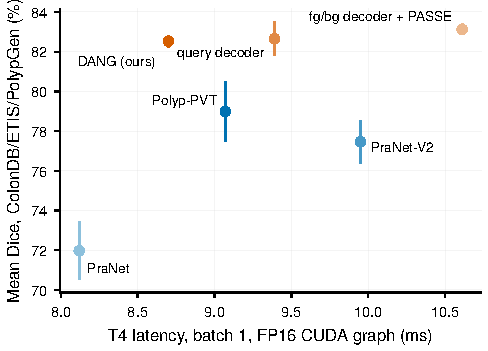
\includegraphics[width=\linewidth]{../figs/accuracy_latency.pdf}
  \caption{\textbf{DANG is more accurate than the retrained models at a comparable latency.} Mean Dice over the three primary cohorts against batch-1 latency on one NVIDIA T4 (FP16 weights, CUDA graph). Points are means over $5$ seeds, bars $95\%$ $t$-intervals of the per-seed mean. Blue: retrained published models; green: SegDINO, timed at its $256\times256$ input; orange: decoders on the DANG encoder and token pyramid.}
  \label{fig:latency}
\end{figure}
\begin{table}[!t]
  \centering
  \caption{\textbf{Inference cost on one NVIDIA T4} at batch size $1$ and $352\times352$ input, all models timed in one process. Params and Trained in millions; MACs per frame in billions; eager: FP16 autocast; graph: FP16 weights replayed from a CUDA graph; throughput at batch size $8$, eager. $^{\S}$: SegDINO is timed at its own $256\times256$ input.}
  \label{tab:eff}
  \vspace{2pt}
  \setlength{\tabcolsep}{3pt}\resizebox{\columnwidth}{!}{%
  \begin{tabular}{l cc c cc c}
    \toprule
    & & & & \multicolumn{2}{c}{\textbf{Latency (ms)}} & \\
    \cmidrule(lr){5-6}
    \textbf{Model} & Params & Trained & GMACs & eager & graph & img/s \\
    \midrule
    \rows{../figs/tab_eff_rows.tex}
    \bottomrule
  \end{tabular}%
  }
\end{table}
Table~\ref{tab:eff} lists the cost of each model, and Figure~\ref{fig:latency} plots accuracy against latency. DANG has the fewest total and trained parameters of all compared models, but about twice the MACs per frame of the Res2Net and PVTv2 models ($25.1$G against $10.8$--$13.0$G), because the frozen encoder runs at $448\times448$. With FP16 weights in a CUDA graph its batch-1 latency ($9.3$~ms, about $107$ frames per second) is below that of Polyp-PVT ($10.1$~ms) and PraNet-V2 ($10.2$~ms) and above that of PraNet ($8.4$~ms). SegDINO, at its $256\times256$ input and with a light head, is the fastest model ($3.7$~ms, $6.9$G MACs), but far less accurate. In eager mode, where the encoder runs in FP32 as in training, DANG has the lowest batch-1 latency of the $352\times352$ models ($22.7$~ms) but the lowest batch-$8$ throughput ($41$ against $155$--$174$ images per second); batched offline processing would need the FP16 encoder.

\section{Limitations}
\label{sec:limits}
\begin{enumerate}
  \item \textbf{Adaptive design.} The standard split has no validation set, and the decoder variants were compared on the test cohorts, including the three primary ones. Kvasir, ClinicDB, ColonDB, ETIS, CVC-300 and PolypGen are therefore not fully held out for DANG. PolypDB was never used for design and was evaluated once, on the final model; it is the only fully held-out result for DANG, and there DANG leads every retrained model, by $3.1$ to $17.5$ points.
  \item \textbf{Recipes differ.} The compared models use the recipes of their papers, DANG its own; in particular only DANG trains with Fourier amplitude mixing and mixed precision. The comparison is between methods as published, not a controlled ablation of the recipe.
  \item \textbf{Hardware.} DANG and most compared models were trained on NVIDIA T4 GPUs; Polyp-PVT, whose $99$-epoch schedule exceeds our T4 session limit, was trained on cloud GPUs of another type.
  \item \textbf{One training split.} All models are trained on the same two centres; we do not test other training sources or label budgets.
  \item \textbf{Scope.} We evaluate single frames, not video, and report no clinical reader study.
\end{enumerate}

\section{Conclusion}
DANG segments polyps from a frozen DINOv3 ViT-S/16 with convolutional adapters, a token pyramid, a scale-aware decoder and a dual-prototype margin head, training $1.9$M of $23.5$M parameters. Retrained under one protocol with five seeds, it ties Polyp-PVT on CVC-ColonDB and exceeds every compared model on ETIS-LaribPolypDB ($+7.3$ points) and PolypGen ($+2.7$ points), and on the held-out PolypDB ($89.8\%$, $+3.1$ points), at a T4 latency of $9.3$~ms, while it trails Polyp-PVT on the in-domain CVC-ClinicDB. All four pyramid levels come from the frozen encoder, without a convolutional backbone, and a heavier fg/bg decoder with a support envelope buys up to $1$ further point at $24\%$ more latency. Next steps are training on other centres, video-level evaluation and a reader study.

\appendices

\section{Implementation Details}
\label{app:impl}

\begin{table*}[!t]
  \centering
  \caption{\textbf{DANG hyperparameters.} Lesion area $a$ is the ground-truth foreground percentage of the image.}
  \label{tab:impl}
  \small
  \begin{tabular}{@{}l p{0.8\textwidth}@{}}
    \toprule
    \textbf{Item} & \textbf{Setting} \\
    \midrule
    Encoder & DINOv3 ViT-S/16 (LVD-1689M), frozen, input $448\times448$, run in FP32 (its attention logits overflow FP16 during training) \\
    Adapters & Conv-LoRA, rank $16$, after each of the $12$ blocks; readout after blocks $3$, $6$, $9$, $12$; $192$ decoder channels \\
    Optimiser & AdamW; learning rate $10^{-3}$ (adapters), $4\times10^{-4}$ (all other trained modules) \\
    Weight decay & $10^{-4}$; none on adapters, normalisation, bias, gain and prototype parameters \\
    Schedule & linear warm-up for $2$ epochs, then cosine decay to $5\%$; $20$ epochs; batch size $16$ \\
    Weight averaging & EMA with decay $\min(0.992,\,(1+t)/(10+t))$ at step $t$; final EMA weights are evaluated \\
    Other & gradient-norm clipping at $3.0$; FP16 mixed precision on T4 \\
    Augmentation & scale $0.65$--$0.90$ ($p=0.3$) or $0.95$--$1.20$ with crop or pad; horizontal and vertical flips ($p=0.5$ each); $90^\circ$ rotations ($p=0.5$); brightness, contrast, saturation $\pm15\%$ ($p=0.4$); hue $\pm0.04$ ($p=0.3$); gamma $0.8$--$1.25$ ($p=0.3$); Fourier amplitude mix with a random batch partner, $\lambda\sim U(0,1)$ ($p=0.5$) \\
    \midrule
    Image weight & $w=\mathrm{clip}\bigl((3/(a+0.35))^{0.4},\,1,\,2.4\bigr)$ \\
    Tversky & false-positive weight $0.45+0.15\,\sigma((a-1.5)/0.5)$, false-negative weight $1$ minus it \\
    Far-field loss & mean probability outside the ground truth dilated by $4$, $8$, $14$ and $20$ pixels \\
    Prototype head & $K=8+8$ prototypes, dimension $128$; $\beta=6$; $\tau$ learned, initialised at $12$ and clamped to $[4,25]$ \\
    & $w_{\text{a}}=10\cdot\tfrac12\tanh(\theta_{\text{a}})$, $w_{\text{ss}}=8\cdot\tfrac12\tanh(\theta_{\text{ss}})$ with learned $\theta$ \\
    Anchors & momentum $0.95$; foreground where pooled mask $\ge0.35$, background where $\le0.10$ \\
    \bottomrule
  \end{tabular}
\end{table*}

\section*{Data and Code Availability}
All experiments use public, de-identified datasets (Kvasir-SEG~\cite{jha2020kvasir}, CVC-ClinicDB, CVC-ColonDB~\cite{tajbakhsh2015automated}, ETIS-LaribPolypDB~\cite{silva2014toward}, CVC-300, PolypGen~\cite{ali2023polypgen} and PolypDB~\cite{jha2024polypdb}) under their research licences; no new patient data were collected. Code, deduplication manifests, per-image evaluation logs and the scripts that regenerate every table from the raw logs will be released.

\section*{Acknowledgment}
The authors would like to express their sincere appreciation to the Vietnam Aerospace University for supporting this research during the 2026--2027 academic year.

\begin{thebibliography}{00}

\bibitem{sung2021globocan} H. Sung, J. Ferlay, R. L. Siegel, M. Laversanne, I. Soerjomataram, A. Jemal, and F. Bray, ``Global cancer statistics 2020: GLOBOCAN estimates of incidence and mortality worldwide for 36 cancers in 185 countries,'' \emph{CA: Cancer J. Clin.}, vol. 71, no. 3, pp. 209--249, 2021.


\bibitem{zauber2012polypectomy} A. G. Zauber \emph{et al.}, ``Colonoscopic polypectomy and long-term prevention of colorectal-cancer deaths,'' \emph{N. Engl. J. Med.}, vol. 366, no. 8, pp. 687--696, 2012.


\bibitem{jha2020kvasir} D. Jha \emph{et al.}, ``Kvasir-SEG: A segmented polyp dataset,'' in \emph{Proc. Int. Conf. MultiMedia Modeling (MMM)}, 2020, pp. 451--462.


\bibitem{fan2020pranet} D.-P. Fan, G.-P. Ji, T. Zhou, G. Chen, H. Fu, J. Shen, and L. Shao, ``PraNet: Parallel reverse attention network for polyp segmentation,'' in \emph{Proc. Med. Image Comput. Comput. Assist. Interv. (MICCAI)}, 2020, pp. 263--273.


\bibitem{tajbakhsh2015automated} N. Tajbakhsh, S. R. Gurudu, and J. Liang, ``Automated polyp detection in colonoscopy videos using shape and context information,'' \emph{IEEE Trans. Med. Imag.}, vol. 35, no. 2, pp. 630--644, Feb. 2016.


\bibitem{silva2014toward} J. Silva, A. Histace, O. Romain, X. Dray, and B. Granado, ``Toward embedded detection of polyps in WCE images for early diagnosis of colorectal cancer,'' \emph{Int. J. Comput. Assist. Radiol. Surg.}, vol. 9, no. 2, pp. 283--293, 2014.


\bibitem{oquab2024dinov2} M. Oquab \emph{et al.}, ``DINOv2: Learning robust visual features without supervision,'' \emph{Trans. Mach. Learn. Res.}, 2024.


\bibitem{simeoni2025dinov3} O. Sim\'{e}oni \emph{et al.}, ``DINOv3,'' 2025, \emph{arXiv:2508.10104}.


\bibitem{yang2025segdino} S. Yang, H. Wang, Z. Xing, S. Chen, and L. Zhu, ``SegDINO: An efficient design for medical and natural image segmentation with DINO-V3,'' 2025, \emph{arXiv:2509.00833}.


\bibitem{ali2023polypgen} S. Ali \emph{et al.}, ``A multi-centre polyp detection and segmentation dataset for generalisability assessment,'' \emph{Sci. Data}, vol. 10, no. 1, Art. no. 75, 2023.


\bibitem{jha2024polypdb} D. Jha \emph{et al.}, ``PolypDB: A curated multi-center dataset for development of AI algorithms in colonoscopy,'' 2024, \emph{arXiv:2409.00045}.


\bibitem{ronneberger2015unet} O. Ronneberger, P. Fischer, and T. Brox, ``U-Net: Convolutional networks for biomedical image segmentation,'' in \emph{Proc. Med. Image Comput. Comput. Assist. Interv. (MICCAI)}, 2015, pp. 234--241.


\bibitem{zhou2018unetplusplus} Z. Zhou, M. M. R. Siddiquee, N. Tajbakhsh, and J. Liang, ``UNet++: A nested U-Net architecture for medical image segmentation,'' in \emph{Proc. Deep Learn. Med. Image Anal. (DLMIA) Workshop}, 2018, pp. 3--11.


\bibitem{lou2022caranet} A. Lou, S. Guan, H. Ko, and M. H. Loew, ``CaraNet: Context axial reverse attention network for segmentation of small medical objects,'' in \emph{Proc. SPIE Med. Imag.}, 2022.


\bibitem{dong2021polyp} B. Dong, W. Wang, D.-P. Fan, J. Li, H. Fu, and L. Shao, ``Polyp-PVT: Polyp segmentation with pyramid vision transformers,'' \emph{CAAI Artif. Intell. Res.}, vol. 2, Art. no. 9150015, 2023, doi: 10.26599/AIR.2023.9150015.


\bibitem{zhang2021transfuse} Y. Zhang, H. Liu, and Q. Hu, ``TransFuse: Fusing transformers and CNNs for medical image segmentation,'' in \emph{Proc. Med. Image Comput. Comput. Assist. Interv. (MICCAI)}, 2021, pp. 14--24.


\bibitem{rahman2024emcad} M. M. Rahman, M. Munir, and R. Marculescu, ``EMCAD: Efficient multi-scale convolutional attention decoding for medical image segmentation,'' in \emph{Proc. IEEE/CVF Conf. Comput. Vis. Pattern Recognit. (CVPR)}, 2024.


\bibitem{hu2026pranetv2} B.-C. Hu, G.-P. Ji, D. Shao, and D.-P. Fan, ``PraNet-V2: Dual-supervised reverse attention for medical image segmentation,'' \emph{Comput. Vis. Media}, 2026, doi: 10.26599/CVM.2025.9450510.


\bibitem{sun2026asgnet} Y. Sun \emph{et al.}, ``ASGNet: Adaptive spectrum guidance network for automatic polyp segmentation,'' \emph{IEEE Trans. Circuits Syst. Video Technol.}, 2026, doi: 10.1109/TCSVT.2026.3685209.


\bibitem{wang2026csgmamba} Y. Wang, J. Wu, J. Song, and S. Ren, ``CSG-Mamba: A convolutional scoring gating vision state space network for endoscopic polyp segmentation,'' 2026, \emph{arXiv:2608.14146}.


\bibitem{urooj2026metrics} A. Urooj, Z. U. Abdien, and N. Madan, ``Metrics or mirage? An audit of evaluation inconsistencies in colonoscopy polyp segmentation benchmarks,'' 2026, \emph{arXiv:2607.08203}.


\bibitem{xi2025fpgm} H. Xi \emph{et al.}, ``Frequency prior guided matching: A data augmentation approach for generalizable semi-supervised polyp segmentation,'' 2025, \emph{arXiv:2508.06517}.


\bibitem{zhou2023samPolyps} T. Zhou, Y. Zhang, Y. Zhou, Y. Wu, and C. Gong, ``Can SAM segment polyps?'' 2023, \emph{arXiv:2304.07583}.


\bibitem{ma2024medsam} J. Ma, Y. He, F. Li, L. Han, C. You, and B. Wang, ``Segment anything in medical images,'' \emph{Nature Commun.}, vol. 15, Art. no. 654, 2024.


\bibitem{jiang2026medsam3} C. Jiang \emph{et al.}, ``Medical SAM3: A foundation model for universal prompt-driven medical image segmentation,'' 2026, \emph{arXiv:2601.10880}.


\bibitem{chen2025sam3adapter} T. Chen \emph{et al.}, ``SAM3-Adapter: Efficient adaptation of Segment Anything 3 for camouflage object segmentation, shadow detection, and medical image segmentation,'' 2025, \emph{arXiv:2511.19425}.


\bibitem{li2026hatsam3} H. L. Li and A. Masood, ``HAT-SAM3: Endoscopy-aware adaptation of a foundation segmentation model for generalizable polyp segmentation,'' \emph{Vis. Comput.}, 2026, doi: 10.1007/s00371-026-04562-3.


\bibitem{dutta2024sammamba} T. K. Dutta, S. Majhi, D. R. Nayak, and D. Jha, ``SAM-Mamba: Mamba guided SAM architecture for generalized zero-shot polyp segmentation,'' 2024, \emph{arXiv:2412.08482}.


\bibitem{dutta2025sammagup} T. K. Dutta, S. Majhi, D. R. Nayak, and D. Jha, ``Mamba guided boundary prior matters: A new perspective for generalized polyp segmentation,'' 2025, \emph{arXiv:2507.01509}.


\bibitem{agnihotri2026litebound} S. Agnihotri, S. Majhi, and D. R. Nayak, ``Sharpening lightweight models for generalized polyp segmentation: A boundary guided distillation from foundation models,'' 2026, \emph{arXiv:2604.17865}.


\bibitem{agnihotri2025difom} S. Agnihotri, S. Majhi, D. R. Nayak, and D. Jha, ``From SAM to DINOv2: Towards distilling foundation models to lightweight baselines for generalized polyp segmentation,'' in \emph{Proc. IEEE/CVF Winter Conf. Appl. Comput. Vis. (WACV)}, 2026, \emph{arXiv:2512.09307}.


\bibitem{agnihotri2026litepi} S. Agnihotri, S. Majhi, D. R. Nayak, D. Mahapatra, and D. Jha, ``Induce to empower: Improving lightweight baselines via foundation model induction for generalized polyp segmentation,'' 2026, \emph{arXiv:2607.17208}.


\bibitem{yang2026segdino} S. Yang \emph{et al.}, ``SegDINO: Introducing multi-scale structure into DINO for efficient medical image segmentation,'' 2026, \emph{arXiv:2606.17972}.


\bibitem{wang2019panet} K. Wang, J. H. Liew, Y. Zou, D. Zhou, and J. Feng, ``PANet: Few-shot image semantic segmentation with prototype alignment,'' in \emph{Proc. IEEE/CVF Int. Conf. Comput. Vis. (ICCV)}, 2019, doi: 10.1109/ICCV.2019.00929.


\bibitem{fan2022ssp} Q. Fan, W. Pei, Y.-W. Tai, and C.-K. Tang, ``Self-support few-shot semantic segmentation,'' in \emph{Proc. Eur. Conf. Comput. Vis. (ECCV)}, 2022, doi: 10.1007/978-3-031-19800-7\_41.


\bibitem{hu2022lora} E. J. Hu \emph{et al.}, ``LoRA: Low-rank adaptation of large language models,'' in \emph{Proc. Int. Conf. Learn. Represent. (ICLR)}, 2022.


\bibitem{zhong2024convlora} Z. Zhong, Z. Tang, T. He, H. Fang, and C. Yuan, ``Convolution meets LoRA: Parameter efficient finetuning for segment anything model,'' in \emph{Proc. Int. Conf. Learn. Represent. (ICLR)}, 2024.


\bibitem{ranftl2021vision} R. Ranftl, A. Bochkovskiy, and V. Koltun, ``Vision transformers for dense prediction,'' in \emph{Proc. IEEE/CVF Int. Conf. Comput. Vis. (ICCV)}, 2021, pp. 12179--12188.


\bibitem{xu2021fact} Q. Xu, R. Zhang, Y. Zhang, Y. Wang, and Q. Tian, ``A Fourier-based framework for domain generalization,'' in \emph{Proc. IEEE/CVF Conf. Comput. Vis. Pattern Recognit. (CVPR)}, 2021, pp. 14383--14392.


\bibitem{wilcoxon1945individual} F. Wilcoxon, ``Individual comparisons by ranking methods,'' \emph{Biometrics Bull.}, vol. 1, no. 6, pp. 80--83, 1945.

\bibitem{holm1979simple} S. Holm, ``A simple sequentially rejective multiple test procedure,'' \emph{Scand. J. Statist.}, vol. 6, no. 2, pp. 65--70, 1979.



\end{thebibliography}

\begin{IEEEbiographynophoto}{Dang Thanh Tuan}
is currently pursuing a B.S. degree in Artificial Intelligence at FPT University, Ho Chi Minh City, Vietnam. His research interests include computer vision, machine learning, data-driven modeling, and AI for scientific discovery. He is particularly interested in developing innovative AI methodologies to address real-world challenges and advance scientific research. He aspires to pursue a Ph.D. degree and contribute to the advancement of these fields.
\end{IEEEbiographynophoto}

\begin{IEEEbiographynophoto}{Phu-Nguyen Le}
received the B.S. degree in electrical engineering from Da Nang University of Science and Technology, Vietnam, in 2012, and the Ph.D. degree from the University of Ulsan, South Korea, in 2021. He is currently a Lecturer with the Faculty of Electrical and Electronics Engineering, Vietnam Aerospace University, Ho Chi Minh City, Vietnam. His research interests include sensor-based robotic applications, robot calibration, and AI-based robotic control.
\end{IEEEbiographynophoto}

\EOD

\end{document}
